\documentclass[12pt,a4paper]{article}

% ============================================================
% PACKAGES
% ============================================================
\usepackage[utf8]{inputenc}
\usepackage[T1]{fontenc}
\usepackage{lmodern}
\usepackage[french]{babel}
\usepackage{geometry}
\usepackage{graphicx}
\graphicspath{{image/}}
\usepackage[table]{xcolor}
\usepackage{listings}
\usepackage{booktabs}
\usepackage{array}
\usepackage{fancyhdr}
\usepackage{titlesec}
\usepackage{enumitem}
\usepackage{mdframed}
\usepackage{tikz}
\usepackage{float}
\usepackage{microtype}
\usepackage{setspace}
\usepackage{hyperref}

% ============================================================
% MISE EN PAGE (plus d'air, lecture confortable)
% ============================================================
\geometry{
  headheight=14pt,
  top=2.6cm,
  bottom=2.8cm,
  left=2.8cm,
  right=2.8cm
}
\setstretch{1.12}

% ============================================================
% COULEURS (palette bleue : lisible, contrastes nets)
% ============================================================
\definecolor{primary}{RGB}{28, 90, 168}
\definecolor{primarylight}{RGB}{88, 145, 220}
\definecolor{secondary}{RGB}{232, 240, 252}
\definecolor{codebg}{RGB}{248, 250, 255}
\definecolor{codeframe}{RGB}{170, 195, 230}
\definecolor{success}{RGB}{34, 130, 90}
\definecolor{warning}{RGB}{200, 120, 40}
\definecolor{darkgray}{RGB}{45, 55, 72}
\definecolor{lightgray}{RGB}{95, 110, 140}

% ============================================================
% EN-TÊTE ET PIED DE PAGE
% ============================================================
\pagestyle{fancy}
\fancyhf{}
\fancyhead[L]{\small\sffamily\textcolor{primary!85!black}{Projet M1 GIL --- Gestion de flotte}}
\fancyhead[R]{\small\sffamily\textcolor{primary!85!black}{Univ. Rouen Normandie · 2025--2026}}
\fancyfoot[C]{\small\sffamily\textcolor{primary!70!black}{\thepage}}
\renewcommand{\headrulewidth}{0.4pt}
\renewcommand{\headrule}{\hbox to\headwidth{\color{primary!35}\leaders\hrule height \headrulewidth\hfill}}
\renewcommand{\footrulewidth}{0pt}

% ============================================================
% STYLE DES TITRES
% ============================================================
\titleformat{\section}
  {\Large\sffamily\bfseries\color{primary}}
  {\thesection.}{0.55em}{}

\titleformat{\subsection}
  {\large\sffamily\bfseries\color{primary!85!black}}
  {\thesubsection.}{0.45em}{}

\titleformat{\subsubsection}
  {\normalsize\sffamily\bfseries\color{primary!75!black}}
  {\thesubsubsection.}{0.4em}{}
\titlespacing*{\section}{0pt}{1.6ex plus .2ex}{1ex plus .1ex}
\titlespacing*{\subsection}{0pt}{1.3ex plus .15ex}{0.7ex plus .1ex}

% ============================================================
% STYLE DU CODE
% ============================================================
\lstset{
  backgroundcolor=\color{codebg},
  frame=single,
  rulecolor=\color{codeframe},
  basicstyle=\ttfamily\footnotesize,
  keywordstyle=\color{primary}\bfseries,
  commentstyle=\color{lightgray}\itshape,
  stringstyle=\color{success},
  breaklines=true,
  showstringspaces=false,
  numbers=left,
  numberstyle=\tiny\sffamily\textcolor{lightgray},
  numbersep=6pt,
  tabsize=2,
  captionpos=b,
  aboveskip=\smallskipamount,
  belowskip=\smallskipamount,
  extendedchars=true,
  keepspaces=true,
  % listings + pdfLaTeX : pas d'accents dans le corps des blocs (sinon erreurs UTF-8)
  literate=
    {á}{{\'a}}1 {é}{{\'e}}1 {è}{{\`e}}1 {à}{{\`a}}1 {ù}{{\`u}}1 {ç}{{\c{c}}}1
    {ô}{{\^o}}1 {î}{{\^i}}1 {ê}{{\^e}}1 {û}{{\^u}}1 {â}{{\^a}}1
    {É}{{\'E}}1 {À}{{\`A}}1 {Ç}{{\c{C}}}1 {œ}{{\oe}}1 {Œ}{{\OE}}1
}

% ============================================================
% BOITE INFO (fond bleu très léger, filet bleu)
% ============================================================
\newmdenv[
  backgroundcolor=secondary,
  linecolor=primary,
  linewidth=1.1pt,
  leftline=true,
  rightline=false,
  topline=false,
  bottomline=false,
  innerleftmargin=11pt,
  innerrightmargin=11pt,
  innertopmargin=9pt,
  innerbottommargin=9pt,
  skipabove=0.6em,
  skipbelow=0.6em
]{infobox}

% Liens PDF
\hypersetup{
  colorlinks=true,
  linkcolor=primary!90!black,
  urlcolor=primarylight,
  citecolor=primary!85!black,
  pdfborderstyle={/S/U/W 0}
}

% ============================================================
% DOCUMENT
% ============================================================
\begin{document}

% ------------------------------------------------------------
% PAGE DE TITRE
% ------------------------------------------------------------
\begin{titlepage}
  \centering
  \vspace*{1cm}

  {\Large\textbf{Université de Rouen Normandie}\\[0.3cm]
  \large Master 1 -- Génie Informatique et Logiciel}

  \vspace{1.5cm}
  {\color{primary!55}\rule{\linewidth}{0.5mm}}\\[0.45cm]

  {\Huge\sffamily\bfseries\color{primary} Projet Gestion de Flotte de véhicules\\[0.35cm]}
  {\LARGE\sffamily\bfseries\color{primary!80!black} Rapport de Semaine 4}\\[0.35cm]
  {\large\sffamily\color{primary!65!black} Microservices Conducteurs \& Maintenance}

  {\color{primary!55}\rule{\linewidth}{0.5mm}}\\[1.5cm]

  \begin{minipage}{0.45\textwidth}
    \begin{flushleft}
      \textbf{Étudiants :}\\
      Ahcene Amouchas \\
      Florian Pepin \\[0.5cm]
      \textbf{Encadrants :}\\
      Lydia \& Luc
    \end{flushleft}
  \end{minipage}
  \hfill
  \begin{minipage}{0.45\textwidth}
    \begin{flushright}
      \textbf{Année universitaire :}\\
      2025 -- 2026 \\[0.5cm]
      \textbf{Semaine :}\\
      4 / 7
    \end{flushright}
  \end{minipage}

  \vfill
  {\large 4 avril 2026}
\end{titlepage}

\tableofcontents
\newpage

% ------------------------------------------------------------
% INTRODUCTION
% ------------------------------------------------------------
\section{Introduction et objectifs de la semaine}

La semaine 4 s'inscrit après la mise en place de l'infrastructure (semaine~2) et le microservice \textbf{Véhicules} (semaine~3). Elle vise à completer la plateforme avec les services \textbf{Conducteurs} et \textbf{Maintenance}, la communication événementielle et la passerelle API, conformément au cahier des charges de la semaine.

\subsection{Objectifs fixés}

Les objectifs pédagogiques et fonctionnels de la semaine~4 sont les suivants :

\begin{itemize}[leftmargin=*]
  \item \textbf{Service Conducteurs :} exposition d'un CRUD complet, \textbf{validation et suivi des permis} (unicité, dates, alertes d'expiration), et \textbf{assignations} véhicule--conducteur cohérentes avec le service Véhicules (y compris via événements).
  \item \textbf{Service Maintenance :} \textbf{planification} des interventions, \textbf{historique} par véhicule, et \textbf{alertes préventives} (échéances, retard, seuils kilométriques).
  \item \textbf{Événements Kafka inter-services :} orchestration légère des transitions d'état et compensations selon un \textbf{pattern Saga} (chorégraphie).
  \item \textbf{API Gateway :} \textbf{agrégation GraphQL} multi-services (Véhicules, Conducteurs, Maintenance) derrière une API unifiée.
  \item \textbf{Authentification :} \textbf{intégration de Keycloak} (JWT, rôles) pour sécuriser les API REST et le Gateway.
\end{itemize}

\begin{infobox}
\textbf{Livrables attendus :} \textbf{trois services communicants} (Véhicules, Conducteurs, Maintenance) et une \textbf{API Gateway opérationnelle} (GraphQL), avec authentification Keycloak et échanges asynchrones Kafka entre services.
\end{infobox}

% ------------------------------------------------------------
% ARCHITECTURE DE PERSISTANCE
% ------------------------------------------------------------
\newpage
\section{Architecture de Persistance}

\begin{infobox}
\textbf{Principe appliqué :} Le pattern \textbf{Database per Service} est respecté strictement. Chaque microservice métier dispose de sa propre instance PostgreSQL (StatefulSet Kubernetes), garantissant une isolation totale des schémas et des données.
\end{infobox}

\subsection{Isolation des instances}

L'architecture de persistance suit le principe \textbf{une base de données par service métier} : chaque microservice dispose de sa propre instance PostgreSQL (StatefulSet) et de son propre nom de base.

\begin{itemize}
    \item \textbf{Véhicules} : \texttt{postgres-vehicle-service} / \texttt{vehicle\_db}.
    \item \textbf{Maintenance} : \texttt{postgres-maintenance-service} / \texttt{maintenance\_db}.
    \item \textbf{Conducteurs} : \texttt{postgres-driver-service} / \texttt{driver\_db}.
\end{itemize}

Les services \textbf{Événements} et \textbf{Localisation} ne sont pas traités dans ce livrable ; leur persistance dédiée sera ajoutée lorsque ces microservices seront développés.

\subsection{Initialisation via Kubernetes}

Les scripts SQL sont fournis via des \textbf{ConfigMaps} distincts, montés dans le bon pod PostgreSQL au \texttt{initdb}. La convention est la \textbf{même pour chaque service} : \texttt{01-<domaine>.sql} pour le schéma (DDL), \texttt{02-<domaine>-seed.sql} pour les données de test ; l'ordre lexicographique garantit le DDL avant les \texttt{INSERT}.

\begin{itemize}
    \item \texttt{vehicle-db-init} : \texttt{01-vehicle.sql}, \texttt{02-vehicle-seed.sql}.
    \item \texttt{maintenance-db-init} : \texttt{01-maintenance.sql}, \texttt{02-maintenance-seed.sql}.
    \item \texttt{driver-db-init} : \texttt{01-driver.sql}, \texttt{02-driver-seed.sql}.
\end{itemize}

\newpage

% ------------------------------------------------------------
% SERVICE DRIVER
% ------------------------------------------------------------
\section{Microservice Driver}

\begin{infobox}
\textbf{Objectif :} Gérer le cycle de vie complet des conducteurs : création de profils, suivi des permis de conduire et de leur validité, et coordination avec le service Véhicules lors des assignations.
\end{infobox}

Le service Driver est implémenté en Java / Spring Boot et déployé sur le port standard \textbf{8080}.

\subsection{Entité Driver et relation avec DriverLicense}

Le modèle de données repose sur une relation \textbf{Un-à-Plusieurs} entre l'entité \texttt{Driver} et \texttt{DriverLicense}. Le service implémente le \textit{Soft Delete} via les annotations Hibernate \texttt{@SQLDelete} et \texttt{@SQLRestriction}, permettant de conserver l'historique tout en masquant les conducteurs désactivés des requêtes courantes.

\begin{lstlisting}[language=Java, caption=Entité Driver avec soft delete Hibernate]
@Entity
@Table(name = "drivers")
@SQLDelete(sql = "UPDATE drivers SET deleted_at = CURRENT_TIMESTAMP WHERE id = ?")
@SQLRestriction("deleted_at IS NULL")
public class Driver {
    @Id
    @GeneratedValue(strategy = GenerationType.UUID)
    private UUID id;

    private String firstName;
    private String lastName;
    private String email;
    private String phone;
    private String employeeId;

    @Enumerated(EnumType.STRING)
    private DriverStatus status = DriverStatus.ACTIVE;

    @OneToMany(mappedBy = "driver", cascade = CascadeType.ALL)
    private List<DriverLicense> licenses = new ArrayList<>();

    private OffsetDateTime deletedAt;
}
\end{lstlisting}

L'entité \texttt{DriverLicense} stocke les informations du permis (numéro, catégorie, date d'émission, date d'expiration, pays) et est liée au conducteur par une clé étrangère. Le champ \texttt{country} a été étendu à 50 caractères (initialement 2) pour accommoder les noms complets de pays.

\subsection{Logique métier et conformité : LicenseScheduler}

Le service Driver intègre une logique de surveillance proactive de la validité des permis. Une tâche planifiée (\texttt{LicenseScheduler}) s'exécute chaque nuit à minuit pour détecter les situations à risque avant qu'elles ne bloquent une opération.

\begin{lstlisting}[language=Java, caption=Vérification proactive des permis (LicenseScheduler)]
@Scheduled(cron = "0 0 0 * * *")
@Transactional(readOnly = true)
public void checkLicenseExpirations() {
    // Détection des permis expirant dans les 30 prochains jours
    LocalDate in30Days = LocalDate.now().plusDays(30);
    licenseRepository.findByExpiryDate(in30Days).forEach(license -> {
        eventProducer.sendLicenseExpiringEvent(license);
    });

    // Détection des permis expirés aujourd'hui
    LocalDate today = LocalDate.now();
    licenseRepository.findByExpiryDate(today).forEach(license -> {
        eventProducer.sendLicenseExpiredEvent(license);
    });
}
\end{lstlisting}

Les événements générés (\texttt{LICENSE\_EXPIRING}, \texttt{LICENSE\_EXPIRED}) sont publiés sur le topic Kafka \texttt{flotte.conducteurs.events} (constant \texttt{DriverEventProducer}) pour notifier les gestionnaires de flotte en temps réel.

\subsection{Endpoints REST du service Driver}

Le service expose une API REST complète en \texttt{snake\_case} accessible via l'Ingress Kubernetes sur le préfixe \texttt{/api/drivers} :

\begin{table}[H]
\centering
\small
\begin{tabular}{|l|l|p{7.5cm}|}
  \hline
  \rowcolor{primary!15}
  \textbf{Méthode} & \textbf{Endpoint} & \textbf{Description} \\
  \hline
  \textbf{GET} & \texttt{/api/drivers} & Liste des conducteurs actifs (filtrable par statut). \\
  \hline
  \textbf{POST} & \texttt{/api/drivers} & Création d'un nouveau profil conducteur. \\
  \hline
  \textbf{GET} & \texttt{/api/drivers/\{id\}} & Détails d'un conducteur par UUID. \\
  \hline
  \textbf{PUT} & \texttt{/api/drivers/\{id\}} & Mise à jour complète du profil. \\
  \hline
  \textbf{PATCH} & \texttt{/api/drivers/\{id\}/status} & Mise à jour du statut (\texttt{active}, \texttt{on\_tour}, etc.). \\
  \hline
  \textbf{POST} & \texttt{/api/drivers/\{id\}/licenses} & Ajout d'un permis de conduire au profil. \\
  \hline
  \textbf{GET} & \texttt{/api/drivers/\{id\}/licenses} & Liste des permis d'un conducteur. \\
  \hline
  \textbf{DELETE} & \texttt{/api/drivers/\{id\}} & Suppression logique du conducteur (Soft Delete). \\
  \hline
\end{tabular}
\caption{Endpoints REST du service Driver}
\end{table}

\newpage

% ------------------------------------------------------------
% SERVICE MAINTENANCE
% ------------------------------------------------------------
\section{Microservice Maintenance}

\begin{infobox}
\textbf{Objectif :} Assurer la traçabilité complète des interventions techniques sur les véhicules de la flotte, de la planification initiale à la clôture, avec détection automatique des retards.
\end{infobox}

\subsection{Entité MaintenanceRecord}

L'entité centrale \texttt{MaintenanceRecord} modélise le cycle de vie d'une intervention technique. Elle utilise plusieurs énumérations (\texttt{MaintenanceType}, \texttt{MaintenanceStatus}, \texttt{MaintenancePriority}) définies en \texttt{SCREAMING\_SNAKE\_CASE} et alignées sur les types ENUM natifs PostgreSQL.

\begin{lstlisting}[language=Java, caption=Entité MaintenanceRecord]
@Entity
@Table(name = "maintenance_records")
public class MaintenanceRecord {
    @Id
    @GeneratedValue(strategy = GenerationType.UUID)
    private UUID id;

    private UUID vehicleId; // Lien logique (pas de FK inter-services)

    @Enumerated(EnumType.STRING)
    private MaintenanceType type; // PREVENTIVE, CORRECTIVE, INSPECTION

    @Enumerated(EnumType.STRING)
    private MaintenanceStatus status = MaintenanceStatus.SCHEDULED;

    @Enumerated(EnumType.STRING)
    private MaintenancePriority priority; // LOW, MEDIUM, HIGH, CRITICAL

    private LocalDate scheduledDate;
    private String description;
    private Double costEur;
    private Integer mileageAtService;
    private Integer nextServiceKm; // Seuil pour les alertes préventives
}
\end{lstlisting}

Le lien vers le service Véhicules est maintenu via un simple UUID (\texttt{vehicleId}) sans clé étrangère inter-bases, conformément aux principes de l'architecture microservices (pas de jointures cross-services).

\newpage
\subsection{Logique Métier et Alertes}

\subsubsection{Détection des retards}

Une tâche planifiée (\texttt{@Scheduled}) s'exécute quotidiennement à 01h00 pour identifier les maintenances dont la date est dépassée et passer leur statut à \texttt{OVERDUE}.

\begin{lstlisting}[language=Java, caption=Tâche de vérification des retards]
@Scheduled(cron = "0 0 1 * * ?")
@Transactional
public void checkOverdueMaintenance() {
    List<MaintenanceRecord> scheduledRecords =
        repository.findByStatus(MaintenanceStatus.SCHEDULED);
    LocalDate today = LocalDate.now();
    for (MaintenanceRecord record : scheduledRecords) {
        if (record.getScheduledDate().isBefore(today)) {
            record.setStatus(MaintenanceStatus.OVERDUE);
            repository.save(record);
            eventProducer.publishAlert(AlertEvent.overdue(
                record.getVehicleId(), "Maintenance en retard"));
        }
    }
}
\end{lstlisting}

\subsubsection{Cloture avec calcul des prochaines échéances}

L'endpoint \texttt{PATCH /api/maintenance/\{id\}/status} permet de clôturer une intervention en renseignant le cout, les notes techniques, le kilométrage au moment de la prestation et le kilométrage de la prochaine échéance. Ces données alimentent les alertes préventives futures.

\subsection{Endpoints REST du service Maintenance}

\begin{table}[H]
\centering
\small
\begin{tabular}{|l|l|p{7.5cm}|}
  \hline
  \rowcolor{primary!15}
  \textbf{Méthode} & \textbf{Endpoint} & \textbf{Description} \\
  \hline
  \textbf{GET} & \texttt{/api/maintenance} & Liste globale, filtrable par véhicule, statut ou priorité. \\
  \hline
  \textbf{POST} & \texttt{/api/maintenance} & Planification d'une nouvelle fiche d'intervention. \\
  \hline
  \textbf{GET} & \texttt{/api/maintenance/vehicle/\{id\}} & Historique complet d'un véhicule. \\
  \hline
  \textbf{PUT} & \texttt{/api/maintenance/\{id\}} & Mise à jour générale de la fiche (description, priorité, date, statut). \\
  \hline
  \textbf{PATCH} & \texttt{/api/maintenance/\{id\}/status} & Cloture technique (cout, kilométrage, notes, prochaine échéance). \\
  \hline
\end{tabular}
\caption{Endpoints REST du service Maintenance}
\end{table}

\newpage

% ------------------------------------------------------------
% TESTS POSTMAN (REST + GraphQL)
% ------------------------------------------------------------
\section{Tests de l'API REST et GraphQL avec Postman}
\label{sec:tests-postman}

\begin{infobox}
\textbf{Objectif :} Valider via Postman les API REST (services Driver et Maintenance, Ingress \texttt{http://flotte.local}) et le Gateway GraphQL (\texttt{/graphql}), avec le même jeton Keycloak pour l'ensemble des scénarios.
\end{infobox}

L'ensemble des tests est organisé dans une collection Postman couvrant trois périmètres : les services REST (Véhicules, Maintenance, Driver) et les requêtes GraphQL. Tous les appels transitent par l'Ingress NGINX du cluster Kubernetes, ce qui valide à la fois la logique applicative et la configuration du routage.

\subsection{Authentification Keycloak}

Avant d'exécuter les requêtes protégées, un token JWT est récupéré auprès du serveur Keycloak via le flux \textit{Client Credentials} :

\begin{lstlisting}[language=bash, caption=Récupération du token Keycloak (client\_credentials)]
POST http://flotte.local/auth/realms/gestion-flotte/protocol/openid-connect/token

Body (x-www-form-urlencoded):
  grant_type    = client_credentials
  client_id     = postman-test
  client_secret = bxBExAzvhcd0U8VI9cQSmxl1fpzNtQxD
\end{lstlisting}

Le token retourné est ensuite injecté automatiquement dans le header \texttt{Authorization: Bearer <token>} de toutes les requêtes suivantes.

\subsection{Scénarios couverts et exemples de corps JSON}

Nous ne détaillons pas un scénario par endpoint : la collection Postman regroupe les requêtes nommées par route ; le tableau~\ref{tab:bilan-postman} synthétise les codes HTTP obtenus. Ci-dessous, quelques corps JSON représentatifs (les autres variantes --- \texttt{PUT}, filtres \texttt{GET}, etc. --- suivent la même structure que dans la collection).

\textbf{Driver.} Ont été validés : création et lecture de profil, \texttt{PUT} complet, \texttt{PATCH} de statut (dont \texttt{ON\_TOUR}), ajout et liste de permis, \texttt{DELETE} logique (Soft Delete Hibernate). Le listing~\ref{lst:postman-driver-post} montre un \texttt{POST} / \texttt{/api/drivers} minimal.

\begin{lstlisting}[language=java, caption=Exemple de corps --- POST \texttt{/api/drivers}, label=lst:postman-driver-post]
{
    "keycloak_user_id": "777a8400-e29b-41d4-a716-446655447777",
    "first_name": "Marc",
    "last_name": "Durand",
    "email": "marc.durand@test.com",
    "phone": "+33799999999",
    "employee_id": "EMP-999"
}
\end{lstlisting}

\textbf{Maintenance.} Ont été validés : création de fiche, listes et historique par véhicule, \texttt{PUT} puis clôture \texttt{PATCH} (coût, kilométrage, événement Kafka \texttt{MAINTENANCE\_COMPLETED}). Le listing~\ref{lst:postman-maint} regroupe un \texttt{POST} de planification et un \texttt{PATCH} de clôture.

\begin{lstlisting}[language=java, caption=Exemples --- POST \texttt{/api/maintenance} et PATCH \texttt{/api/maintenance/\{id\}/status}, label=lst:postman-maint]
// POST : planification
{ "vehicle_id": "39e75ab3-7878-48a4-814e-f20c63fc99b7",
  "type": "CORRECTIVE", "priority": "HIGH",
  "scheduled_date": "2026-05-01", "description": "Changement des pneus" }

// PATCH : cloture (couts, notes, km)
{ "status": "COMPLETED", "cost_eur": 250.50,
  "notes": "Tout est OK, plaquettes changees.",
  "mileage_at_service": 45000,   "next_service_km": 60000 }
\end{lstlisting}

\subsection{Bilan des tests REST}

\begin{table}[H]
\centering
\small
\begin{tabular}{|l|l|l|l|}
  \hline
  \rowcolor{primary!15}
  \textbf{Service} & \textbf{Endpoint} & \textbf{Code attendu} & \textbf{Résultat} \\
  \hline
  Driver & POST /api/drivers & 201 Created & \textcolor{success}{\textbf{OK}} \\
  Driver & GET /api/drivers & 200 OK & \textcolor{success}{\textbf{OK}} \\
  Driver & GET /api/drivers/\{id\} & 200 OK & \textcolor{success}{\textbf{OK}} \\
  Driver & PUT /api/drivers/\{id\} & 200 OK & \textcolor{success}{\textbf{OK}} \\
  Driver & PATCH /api/drivers/\{id\}/status & 200 OK & \textcolor{success}{\textbf{OK}} \\
  Driver & POST /api/drivers/\{id\}/licenses & 201 Created & \textcolor{success}{\textbf{OK}} \\
  Driver & GET /api/drivers/\{id\}/licenses & 200 OK & \textcolor{success}{\textbf{OK}} \\
  Driver & DELETE /api/drivers/\{id\} & 204 No Content & \textcolor{success}{\textbf{OK}} \\
  \hline
  Maintenance & POST /api/maintenance & 201 Created & \textcolor{success}{\textbf{OK}} \\
  Maintenance & GET /api/maintenance & 200 OK & \textcolor{success}{\textbf{OK}} \\
  Maintenance & GET /api/maintenance/vehicle/\{id\} & 200 OK & \textcolor{success}{\textbf{OK}} \\
  Maintenance & PUT /api/maintenance/\{id\} & 200 OK & \textcolor{success}{\textbf{OK}} \\
  Maintenance & PATCH /api/maintenance/\{id\}/status & 200 OK & \textcolor{success}{\textbf{OK}} \\
  \hline
\end{tabular}
\caption{Bilan des 13 endpoints testés --- Services Driver et Maintenance}
\label{tab:bilan-postman}
\end{table}

L'ensemble des 13 endpoints testés retournent les codes HTTP attendus. Le Soft Delete Hibernate est correctement implémenté sur le service Driver. La clôture d'une intervention de maintenance déclenche bien la mise à jour du statut véhicule via Kafka, validant l'intégration inter-services.

\subsection{Requêtes GraphQL testées via Postman}
\label{sec:postman-graphql}

Les tests manuels reprennent le même jeton Keycloak que pour les API REST : requêtes \texttt{POST} vers \texttt{/graphql} sur l'Ingress (\texttt{http://flotte.local}), corps JSON au format GraphQL. Ont été validées des \textbf{queries de lecture} sur les trois domaines : liste des véhicules (\texttt{vehicles}), fiches de maintenance paginées (\texttt{maintenanceRecords} avec \texttt{items}), liste des conducteurs (\texttt{drivers} avec \texttt{items}), avec les champs utiles (identifiants, statuts, métadonnées). Les réponses renvoient un JSON conforme au schéma, sans erreur dans le tableau \texttt{errors} pour ces scénarios.

\subsection{Bilan des tests GraphQL}

\begin{table}[H]
\centering
\small
\begin{tabular}{|l|l|l|l|}
  \hline
  \rowcolor{primary!15}
  \textbf{Domaine} & \textbf{Opération testée} & \textbf{Réponse HTTP} & \textbf{Résultat} \\
  \hline
  Véhicules & Query \texttt{vehicles} (liste, champs principaux) & 200 OK & \textcolor{success}{\textbf{OK}} \\
  \hline
  Maintenance & Query \texttt{maintenanceRecords} (\texttt{items}, filtres de base) & 200 OK & \textcolor{success}{\textbf{OK}} \\
  \hline
  Conducteurs & Query \texttt{drivers} (\texttt{items}, profils) & 200 OK & \textcolor{success}{\textbf{OK}} \\
  \hline
\end{tabular}
\caption{Bilan des requêtes GraphQL validées via Postman (Gateway, JWT Ingress).}
\label{tab:bilan-graphql}
\end{table}

Ces trois requêtes couvrent les resolveurs racine exposés par le Gateway ; les enchaînements d'agrégation (relations entre types) sont présentés section~\ref{sec:graphql-aggregation}.

\newpage

% ------------------------------------------------------------
% GRAPHQL GATEWAY
% ------------------------------------------------------------
\section{Exposition via le Gateway GraphQL}

\begin{infobox}
\textbf{Objectif :} Remplacer les stubs de la semaine 3 par les résolveurs opérationnels des services Driver et Maintenance, et activer l'agrégation multi-services.
\end{infobox}

\subsection{Architecture du Gateway (Apollo Server)}

Le Gateway GraphQL est une application Node.js dédiée, buildée dans une image Docker \texttt{graphql-gateway:latest} et déployée sur le port 4000 du cluster Kubernetes. Les requêtes sont résolues via un \texttt{Context} instanciant des clients REST (Axios) qui injectent systématiquement le jeton d'authentification reçu :

\begin{itemize}
    \item \textbf{VehicleClient} : requêtes vers \texttt{http://vehicle-service:8080}
    \item \textbf{DriverClient} : requêtes vers \texttt{http://driver-service:8080}
    \item \textbf{MaintenanceClient} : requêtes vers \texttt{http://maintenance-service:8080}
\end{itemize}

La configuration de l'\textbf{Ingress} route le trafic de \texttt{/graphql} vers cette passerelle. Une correction du header \texttt{Authorization} a été apportée pour que le JWT soit systématiquement transmis aux services backend.

\subsection{Résolveurs opérationnels}

Les trois familles de resolveurs sont désormais pleinement fonctionnelles. Le fichier \texttt{index.ts} assemble les resolveurs par spread operator : les nouvelles entrées écrasent les stubs correspondants sans modifier la structure d'agrégation. Les tests Postman sur les queries racine et le tableau de résultats sont décrits section~\ref{sec:postman-graphql}.

\subsection{Agrégation multi-services}
\label{sec:graphql-aggregation}

L'API Gateway permet d'agréger les données de façon transparente pour le client. Les relations suivantes sont désormais résolubles en une seule requête GraphQL :

\begin{itemize}
    \item \textbf{Véhicule $\leftrightarrow$ Maintenance} : Affichage de l'historique technique depuis la fiche véhicule.
    \item \textbf{Véhicule $\leftrightarrow$ Conducteur} : Détail de l'assignation courante d'un véhicule vers le profil du conducteur (et ses permis).
    \item \textbf{Maintenance $\leftrightarrow$ Conducteur} : Résolution du technicien assigné à une intervention.
\end{itemize}

\newpage

% ------------------------------------------------------------
% SAGA PATTERN
% ------------------------------------------------------------
\section{Architecture événementielle (Saga Pattern)}

\begin{infobox}
\textbf{Principe :} Le pattern Saga par \textbf{Chorégraphie} assure la cohérence éventuelle entre les services sans orchestrateur central. Chaque service réagit aux événements publiés par les autres et publie à son tour ses propres événements de résultat.
\end{infobox}

\subsection{Format d'enveloppe unifié (KafkaEventEnvelope)}

Tous les événements inter-services partagent un format d'enveloppe standardisé, facilitant le traçage et l'audit :

\begin{lstlisting}[language=java, caption=Format KafkaEventEnvelope unifié]
{
  "eventId": "625c87b9-...",
  "eventType": "MAINTENANCE_COMPLETED",
  "timestamp": 1775220800.293,
  "payload": {
    "record_id": "7e3638d7-...",
    "vehicle_id": "39e75ab3-...",
    "cost_eur": 250.50
  },
  "metadata": { "triggered_by": "maintenance-service" }
}
\end{lstlisting}

\subsection{Transactions Compensatoires (Cycle de Maintenance)}

Pour garantir l'intégrité des données lors d'une transition d'état impliquant plusieurs services, un mécanisme de compensation a été mis en œuvre :

\begin{enumerate}
    \item \textbf{T1 (Action)} : Le service Maintenance crée une fiche (\texttt{MAINTENANCE\_SCHEDULED}) ; lors du passage en \texttt{IN\_PROGRESS}, il publie \texttt{MAINTENANCE\_STARTED} sur \texttt{flotte.maintenance.events}.
    \item \textbf{T2 (Réaction)} : Le service Véhicule consomme \texttt{MAINTENANCE\_STARTED} et tente de passer le véhicule en \texttt{in\_maintenance}.
    \item \textbf{C1 (Compensation)} : En cas d'échec, le service Véhicule publie \texttt{MAINTENANCE\_REJECTED}. Le service Maintenance consomme cet événement et appelle \texttt{cancelRecord} (statut \texttt{CANCELLED}, note de traçabilité).
\end{enumerate}

\subsection{Topics Kafka et flux d'événements}

\subsubsection{Topic : flotte.maintenance.events}

Le service Véhicules consomme ces messages pour ajuster l'état opérationnel du parc :
\begin{itemize}
    \item \texttt{MAINTENANCE\_STARTED} $\rightarrow$ Statut véhicule : \texttt{in\_maintenance}.
    \item \texttt{MAINTENANCE\_COMPLETED} / \texttt{MAINTENANCE\_CANCELLED} $\rightarrow$ Statut véhicule : \texttt{available}.
\end{itemize}

\subsubsection{Topic : flotte.conducteurs.events}

Ce topic centralise les événements du cycle de vie des conducteurs :
\begin{itemize}
    \item \texttt{DRIVER\_CREATED} / \texttt{DRIVER\_UPDATED} : Notifient les autres services des changements de profil.
    \item \texttt{LICENSE\_EXPIRING} / \texttt{LICENSE\_EXPIRED} : Alertes proactives générées par le \texttt{LicenseScheduler}.
\end{itemize}

\subsubsection{Topic : flotte.assignments.events (flux Véhicule $\rightarrow$ Driver)}

Le service Driver écoute ce topic : sur \texttt{VEHICLE\_ASSIGNED}, le conducteur passe en \texttt{ON\_TOUR} ; sur \texttt{VEHICLE\_UNASSIGNED}, il repasse en \texttt{ACTIVE}. Ces événements sont publiés par le service Véhicules lors des assignations / désassignations, sans appel REST direct entre les deux services.

\subsection{Flux de données}

L'architecture repose sur deux modes de communication complémentaires :

\begin{itemize}
    \item \textbf{Flux synchrones (Gateway GraphQL)} : Les requêtes de lecture transitent par le Gateway qui appelle en parallèle les services REST concernés et assemble les réponses JSON en un objet unifié.
    \item \textbf{Flux asynchrones (Kafka)} : Les changements d'état critiques (cycle de vie Maintenance, mise à jour kilométrique, assignation conducteur) utilisent le bus de messages pour garantir le découplage et la cohérence éventuelle.
\end{itemize}

\subsection{Remarque sur l'Outbox Pattern}

Une réflexion a été conduite sur la fiabilité de la double écriture (base de données + Kafka). L'\textbf{Outbox Pattern} constitue le standard industriel pour garantir l'atomicité parfaite entre persistance et publication d'événements. Toutefois, compte tenu de la complexité opérationnelle qu'implique un outil comme \textit{Debezium}, nous avons opté pour le \textbf{Direct Publishing} au sein de transactions Spring \texttt{@Transactional}. Cette approche, combinée aux transactions compensatoires du Saga, offre un excellent compromis robustesse/maintenabilité pour notre périmètre.

\newpage

% ------------------------------------------------------------
% TESTS AUTOMATISES
% ------------------------------------------------------------
\section{Tests automatisés et couverture de code}

\begin{infobox}
\textbf{Objectif :} Garantir la robustesse via une couverture minimale de \textbf{80\% en lignes de code} sur les tests \textbf{unitaires} des trois services métier (\textbf{vehicle-service}, \textbf{maintenance-service}, \textbf{driver-service}), mesurée avec JaCoCo.
\end{infobox}

\subsection{Stratégie de tests}

L'approche de test couvre le périmètre métier via deux niveaux complémentaires :

\begin{itemize}
    \item \textbf{Tests unitaires (JUnit 5 + Mockito, \texttt{@WebMvcTest} pour les contrôleurs)} : validation des services, producteurs/consommateurs Kafka mockés, et endpoints REST sans lever tout le contexte Spring sauf pour les tranches nécessaires.
    \item \textbf{Tests d'intégration (\texttt{@SpringBootTest}, MockMvc, base H2 en profil \texttt{test})} : chargement du contexte applicatif, vérification des flux HTTP et de la persistance sur une base embarquée.
\end{itemize}

\subsection{Mesure JaCoCo : profil Maven \texttt{unit-coverage}}

La couverture demandée pour le cours porte sur les \textbf{tests unitaires} uniquement. Nous avons donc ajouté un profil Maven \texttt{unit-coverage} dans chaque service : Surefire \textbf{exclut} les classes \texttt{*IntegrationTest}, le dossier \texttt{intégration/} et les tests de chargement de contexte \texttt{*ApplicationTests}, afin que JaCoCo ne comptabilise pas ces exécutions dans le rapport ``unitaire''.

\textbf{Génération du rapport HTML} (à exécuter dans le répertoire du service concerné, par ex.\ \texttt{services/driver-service/}) :

\begin{lstlisting}[language=bash, caption=Commandes Maven (Wrapper) pour la couverture unitaire]
./mvnw clean test -Punit-coverage
\end{lstlisting}

Le rapport est alors produit sous \texttt{target/site/jacoco/index.html} (un rapport par module). Chaque exécution \textbf{régénère} ce dossier : pour conserver la mesure ``uniquement unitaire'', il faut lancer la commande ci-dessus avec le profil \texttt{unit-coverage} avant de capturer les captures d'écran.

\textbf{Vérification du seuil à 80\% (lignes)} en phase \texttt{verify} (optionnel, fait échouer la build si le seuil n'est pas atteint) :

\begin{lstlisting}[language=bash, caption=Vérification JaCoCo avec seuil minimal]
./mvnw clean verify -Punit-coverage -Djacoco.skip.unit.check=false
\end{lstlisting}

Par défaut, le \texttt{jacoco:check} du profil est \textbf{désactivé} (\texttt{jacoco.skip.unit.check=true}) pour ne pas bloquer le développement ; passer \texttt{jacoco.skip.unit.check=false} active la contrainte.

\newpage
\subsection{Rapports JaCoCo captures (les trois services)}

Les figures~\ref{fig:jacoco-driver} à~\ref{fig:jacoco-vehicle} présentent la vue d'ensemble JaCoCo pour chaque service, obtenue après \texttt{./mvnw clean test -Punit-coverage}. Les fichiers sources des captures sont stockés dans le répertoire \texttt{docs/rapport-S4/image/} (\texttt{jacoco-driver.png}, \texttt{jacoco-maintenance.png}, \texttt{jacoco-vehicle.png}).

\begin{figure}[H]
  \centering
  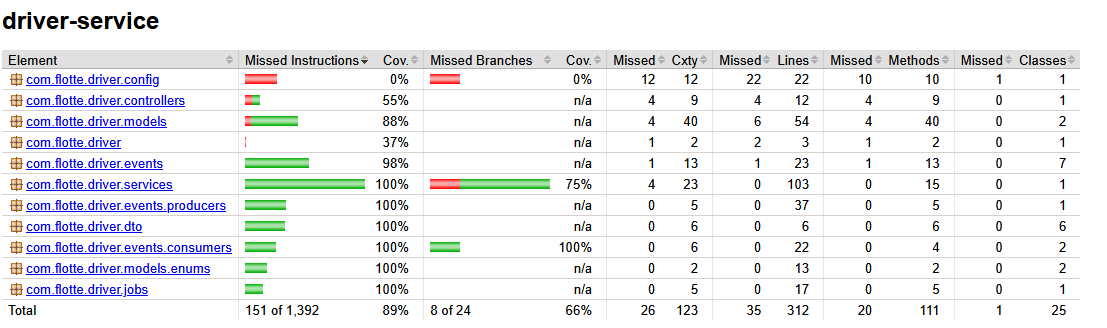
\includegraphics[width=\textwidth]{./image/driver-jacoco.png}
  \caption{Rapport JaCoCo (vue globale) --- \texttt{driver-service}, couverture sur tests unitaires (\texttt{-Punit-coverage}).}
  \label{fig:jacoco-driver}
\end{figure}

\begin{figure}[H]
  \centering
  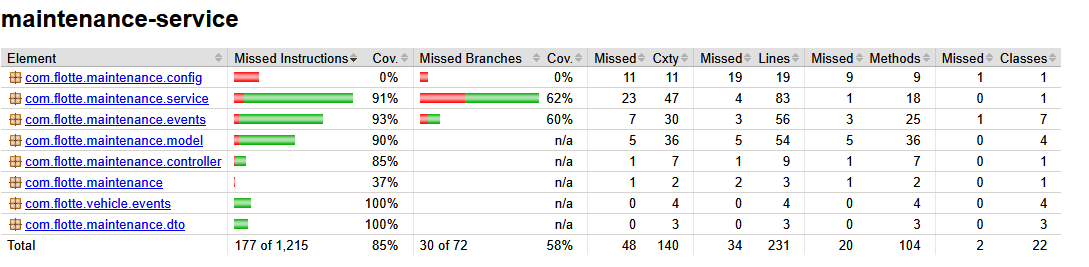
\includegraphics[width=\textwidth]{./image/maintenance-jacoco.png}
  \caption{Rapport JaCoCo (vue globale) --- \texttt{maintenance-service}, couverture sur tests unitaires (\texttt{-Punit-coverage}).}
  \label{fig:jacoco-maintenance}
\end{figure}

\begin{figure}[H]
  \centering
  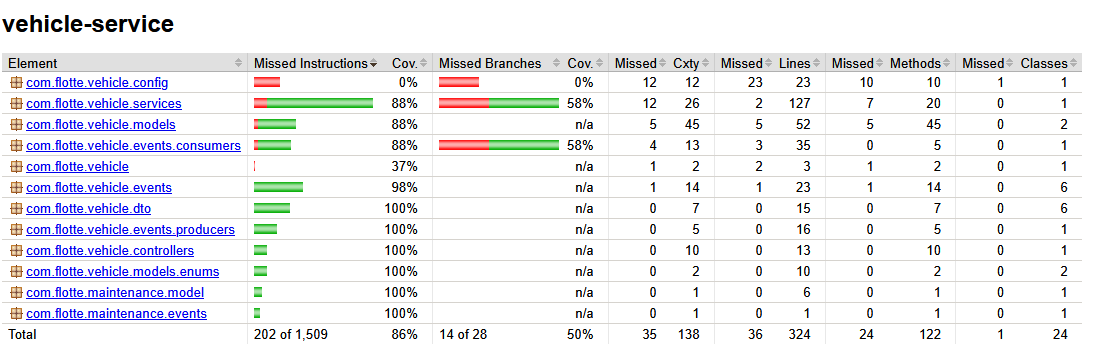
\includegraphics[width=\textwidth]{./image/vehicule-jacoco.png}
  \caption{Rapport JaCoCo (vue globale) --- \texttt{vehicle-service}, couverture sur tests unitaires (\texttt{-Punit-coverage}).}
  \label{fig:jacoco-vehicle}
\end{figure}

\subsection{Synthèse des résultats (tests unitaires, métrique \textbf{lignes})}

Après exécution de \texttt{./mvnw clean test -Punit-coverage} et analyse des rapports, les trois services dépassent le seuil de 80\% en couverture de \textbf{lignes} sur le bundle (packages applicatifs). Les pourcentages exacts peuvent varier légèrement selon l'évolution du code ; les figures ci-dessus font foi au moment du rapport.

\begin{table}[H]
\centering
\small
\begin{tabular}{|l|l|l|}
  \hline
  \rowcolor{primary!15}
  \textbf{Service} & \textbf{Couverture lignes (ordre de grandeur)} & \textbf{Objectif} \\
  \hline
  \texttt{driver-service} & $\approx$ 89\% & $\geq$ 80\% \\
  \texttt{maintenance-service} & $\approx$ 85\% & $\geq$ 80\% \\
  \texttt{vehicle-service} & $\approx$ 89\% & $\geq$ 80\% \\
  \hline
\end{tabular}
\caption{Synthèse indicative (profil \texttt{unit-coverage}, métrique lignes JaCoCo).}
\end{table}

La couverture de \textbf{branches} reste plus basse sur certains modules (consommateurs Kafka, chemins d'erreur), ce qui est classique ; l'exigence du module a été exprimée sur les \textbf{lignes} via le \texttt{jacoco:check} du profil.

\end{document}